% Preamble: \usepackage{amsmath,amssymb,graphicx,algorithm,algpseudocode}
% Upload this directory to Overleaf; input this file from the manuscript.
\section{Joint Optimization of Modulation Variance and Maxwell--Boltzmann Shaping Parameter}
\label{sec:joint-modulation-optimization}

Modulation variance and probability shaping jointly determine the coherent-state
ensemble seen by the mutual-information and security calculations. Optimizing
mutual information alone is therefore insufficient: a modulation change can
also change Eve's Holevo information. We optimize the unchanged asymptotic
reverse-reconciliation objective
\begin{equation}
 K(L,\nu_{\rm MB},V_A)=0.95I_{AB}(L,\nu_{\rm MB},V_A)
 -\chi_{BE}(L,\nu_{\rm MB},V_A;Z_-).
 \label{eq:joint-skr-objective}
\end{equation}
The same normalized 256-state ensemble and channel excess noise enter both
terms. Here $\nu_{\rm MB}$ denotes the raw MB parameter of the stored square-QAM
convention; the internal repository parameter is
$\nu_{\rm repo}=42.5\nu_{\rm MB}$. The intended problem is
\begin{equation}
 \max_{\nu_{\rm MB}\ge0,\,V_A>0} K(L,\nu_{\rm MB},V_A).
 \label{eq:joint-modulation-problem}
\end{equation}
The maintained numerical AO implementation uses strictly positive $\nu_{\rm MB}$.
The difference at the uniform endpoint is an unresolved domain-coverage issue,
not a change to Eq.~\eqref{eq:joint-modulation-problem}.

\subsection{Alternating-coordinate implementation}
For outer iteration $r$, P1 fixes the preceding shaping parameter and P2 fixes
the newly selected variance:
\begin{align}
 V_A^{(r)}&\approx\arg\max_{V_A>0}
 K(L,\nu_{\rm MB}^{(r-1)},V_A),\label{eq:p1}\\
 \nu_{\rm MB}^{(r)}&\approx\arg\max_{\nu_{\rm MB}>0}
 K(L,\nu_{\rm MB},V_A^{(r)}).\label{eq:p2}
\end{align}
The approximation signs denote the actual finite numerical coordinate searches,
not analytically solved subproblems. Algorithm~\ref{alg:ao} describes the
implemented updates. Each search considers all available exact points on its
slice, expands an improving endpoint by halving or doubling, and requests paired
midpoints around an interior best point. Unavailable moments or invalid
evaluations are recorded, never filled by interpolation.

The maintained initial shaping parameters are $0.1$, $0.15$, $0.3$, and $0.8$.
Except for an available supplied warm-start variance, a start uses the smallest
available positive variance on its slice. For subsequent distances, the
preceding selected pair is appended as a warm start. The valid terminal result
with the largest recorded SKR is selected; this selection is separately checked
against the complete compatible finite catalog.

The original limits remain six outer iterations, four inner refinement stages
and three boundary-expansion attempts. The objective tolerance is
$10^{-8}$ bits/use and the coordinate-radius tolerance is $10^{-6}$.
The algorithm checks objective change together with actual coordinate status.
A flat trajectory with missing moments is reported as catalog stagnation; an
open direction is reported as an unresolved boundary. Numerical stopping also
requires both coordinate searches to be complete and no unresolved search earlier
in that start. Neither stopping nor local bracketing proves global optimality.

% Preamble: \usepackage{algorithm,algpseudocode,amsmath,amssymb}
% nu_MB denotes nu_raw; these are approximate finite coordinate searches.
\begin{algorithm}[t]
\caption{Exact-source alternating optimization with explicit search status}
\label{alg:ao}
\small
\begin{algorithmic}[1]
\Require Frozen channel configuration $\mathcal C$, distance $L$, compatible
source/objective cache; starts $(\nu_0,V_{A,0})$; optional previous-distance
solution; $\epsilon_K=10^{-8}$, $\epsilon_p=10^{-6}$,
$R=6$, $J=4$, $B=3$
\Ensure Best recorded $(\nu_{\rm MB}^{\rm best},V_A^{\rm best},K_{\rm best})$
and termination/validation status
\State Form starts $\nu_0\in\{0.1,0.15,0.3,0.8\}$; append the previous-distance pair when available
\For{each start $(\nu_0,V_{A,0})$}
  \State Use $V_{A,0}$ if it is an available exact value on this slice; otherwise use the smallest available positive $V_A$
  \State Initialize $x=(\nu_0,V_A)$ and $K(x)$; skip the start if initialization is unavailable or invalid
  \State $u\gets\mathrm{false}$; $s\gets\texttt{MAX\_ITERATIONS\_REACHED}$
  \For{$r=1,\ldots,R$}
    \State $x_{\rm old}\gets x$, $K_{\rm old}\gets K(x)$
    \State $q_1\gets\Call{CoordinateSearch}{V_A,\nu_{\rm old},\epsilon_K,\epsilon_p,J,B}$
    \State Stop this start with the corresponding failure status if $q_1$ has no valid best point
    \State $\widetilde V_A\gets q_1.\mathrm{best}.V_A$ \Comment{P1 update}
    \State $q_2\gets\Call{CoordinateSearch}{\nu_{\rm MB},\widetilde V_A,\epsilon_K,\epsilon_p,J,B}$
    \State Stop this start with the corresponding failure status if $q_2$ has no valid best point
    \State $x\gets(q_2.\mathrm{best}.\nu_{\rm MB},\widetilde V_A)$; $K(x)\gets q_2.\mathrm{best}.K$
    \State Record P1/P2 parameters, objective values, candidate events and search statuses
    \State $u\gets u\lor\neg(\Call{Closed}{q_1}\land\Call{Closed}{q_2})$
    \State $\Delta K\gets K(x)-K_{\rm old}$
    \If{nonfinite $\Delta K$, $\Delta K<-\epsilon_K$, a monotonicity warning, or recorded numerical failures}
      \State $s\gets\texttt{NUMERICAL\_FAILURE}$; \textbf{break}
    \ElsIf{$|\Delta K|\le\epsilon_K$}
      \If{either coordinate has an unclosed boundary}
        \State $s\gets\texttt{UNRESOLVED\_BOUNDARY}$
      \ElsIf{$u$ or either coordinate is incomplete}
        \State $s\gets\texttt{STAGNATED\_IN\_EXACT\_CATALOG}$
      \Else
        \State $s\gets\texttt{CONVERGED\_NUMERICALLY}$
      \EndIf
      \State \textbf{break}
    \EndIf
  \EndFor
  \State Retain the last complete P1--P2 update and its status $s$
\EndFor
\State Select the valid terminal result with largest recorded $K$; break ties by existing start order
\State Independently compare with the largest compatible catalog value and report coordinate/global-optimality limitations
\end{algorithmic}
\end{algorithm}

\noindent\textbf{Implemented coordinate search.}
\textsc{CoordinateSearch} first evaluates every available positive value on the
fixed-coordinate slice, without interpolation, and selects the largest valid
objective. If the winner is an endpoint, it tests half or twice that parameter,
respectively, with at most three expansion attempts. Missing or invalid points
remain explicit events. A successful outer test must leave the winner between
evaluated neighbors; one tested side of a singleton does not close both sides.
For an interior winner $z$ with nearest evaluated neighbors $z_-<z<z_+$,
the routine checks
$\max(z-z_-,z_+-z)\le10^{-6}$ at loop entry. Otherwise it requests
$(z_-+z)/2$ and $(z+z_+)/2$, in that order, and selects the best of all valid
points. A stage is counted as attempted even when a midpoint is unavailable;
at most four stages are attempted. Reaching the cap is not closure. In
particular, the code does not perform an additional tolerance check after the
fourth stage. \textsc{Closed} requires
\texttt{NUMERICALLY\_CLOSED\_LOCAL\_BRACKET}, no missing source moments,
no numerical failures, and no open boundary. The unresolved flag is persistent
within a start, so an earlier incomplete search prevents a later flat objective
from being labeled numerical convergence.

\noindent\textbf{Scope.} The implementation searches $\nu_{\rm MB}>0$,
$V_A>0$. The theoretical MB family also includes $\nu_{\rm MB}=0$; that
endpoint is not added silently. These finite approximate coordinate searches
are not exact continuous argmax operations or a global-optimality certificate.


\subsection{Validated numerical results}
The current compatible catalog contains 147 distinct MB source pairs and
3,822 stored objective evaluations over 26 distances. The genuine historical
AO records contain 129 multi-start runs and 283 outer iterations. Independent
ranking of every distance's 147 stored values reproduces the AO-selected
finite-catalog maximum at all 26 distances. These are finite-set best-found
results, not continuous globally optimal values.
This agreement concerns selection of the best terminal result across starts,
not convergence of every start: 59 of the 129 individual terminal results
attain their distance's catalog maximum, and no distance has unanimous
agreement among all its starts. The recorded terminal states comprise 20
catalog-stagnation and 109 unresolved-boundary cases. Multi-start selection
is therefore important for the reported best-found curve.

At $L=21.9393102292$ km, the best recorded pair and its decomposition are
\begin{align}
 (\nu_{\rm MB}^{\rm best},V_A^{\rm best})&=(0.165,5.5),\nonumber\\
 I_{AB}&=0.6341892631163653,\nonumber\\
 0.95I_{AB}&=0.602479799960547,\nonumber\\
 \chi_{BE}&=0.5244988060866094,\nonumber\\
 K_{\rm best}&=0.07798099387393764\ \text{bits/use}.
\end{align}
The nearest evaluated variance neighbors $5.4875$ and $5.5125$, at fixed
$\nu_{\rm MB}=0.165$, have SKR values $0.07798091552916897$ and
$0.07798086747835642$, respectively. They support the incumbent among these
evaluated neighbors, but do not locate an unmeasured continuous maximum.
The runner-up gap is approximately $7.83448\times10^{-8}$ bits/use; a complete
objective-error bound at that scale has not been established.

Four of the five starts at this distance, including the warm start, reach the
same recorded pair. The $\nu_0=0.8$ start follows the complete-cycle sequence
$(0.8,1.5)\to(0.5,1.5)\to(0.4,3.0)\to(0.4,3.0)$ and ends at
$K=0.06912585821984563$ bits/use. Its final P1 and P2 requests lack moments
at $(0.4,1.5)$ and $(0.2,3.0)$, respectively. Its lower terminal value therefore
demonstrates sensitivity to finite exact-source coverage, not evidence for a
distinct converged basin. Figures~\ref{fig:ao-history} and
\ref{fig:ao-parameters} show only genuine recorded updates.

At $22$ km the catalog best is $(0.165,5.475)$ with
$K=0.07661740491526092$ bits/use. Its exact fixed-variance shaping slice has only
one available point, so the associated coordinate search cannot be considered
closed. The complete parameter and metric table is supplied as
\texttt{optimized\_skr\_26\_distances.csv}.

\begin{figure}[t]
 \centering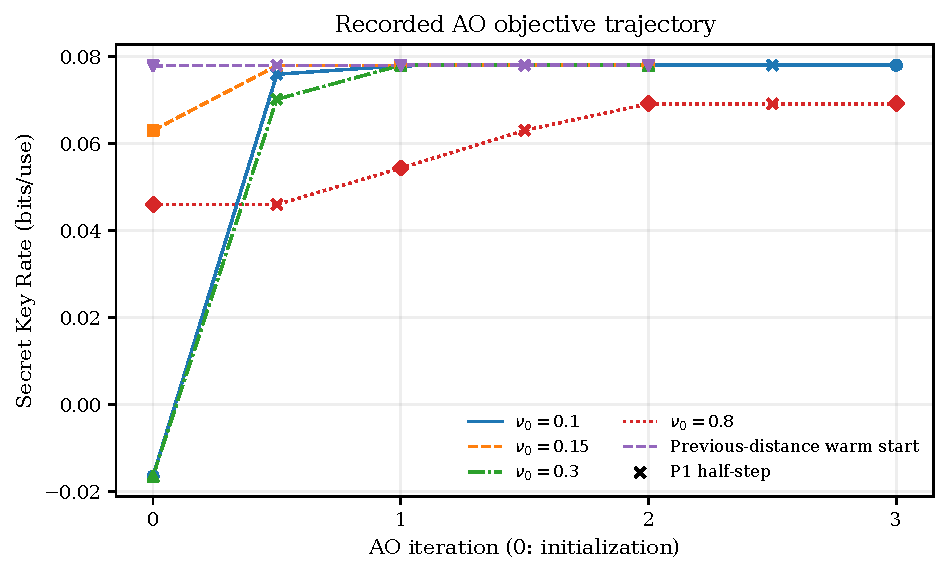
\includegraphics[width=\linewidth]{ao_convergence.pdf}
 \caption{Recorded AO objective histories at $L=21.9393102292$ km.
 Initialization is iteration zero; crosses show recorded P1 half-steps and
 markers at integer iterations show complete P1--P2 cycles. Flat portions
 accompany incomplete searches and are not a numerical-convergence certificate.}
 \label{fig:ao-history}
\end{figure}
\begin{figure}[t]
 \centering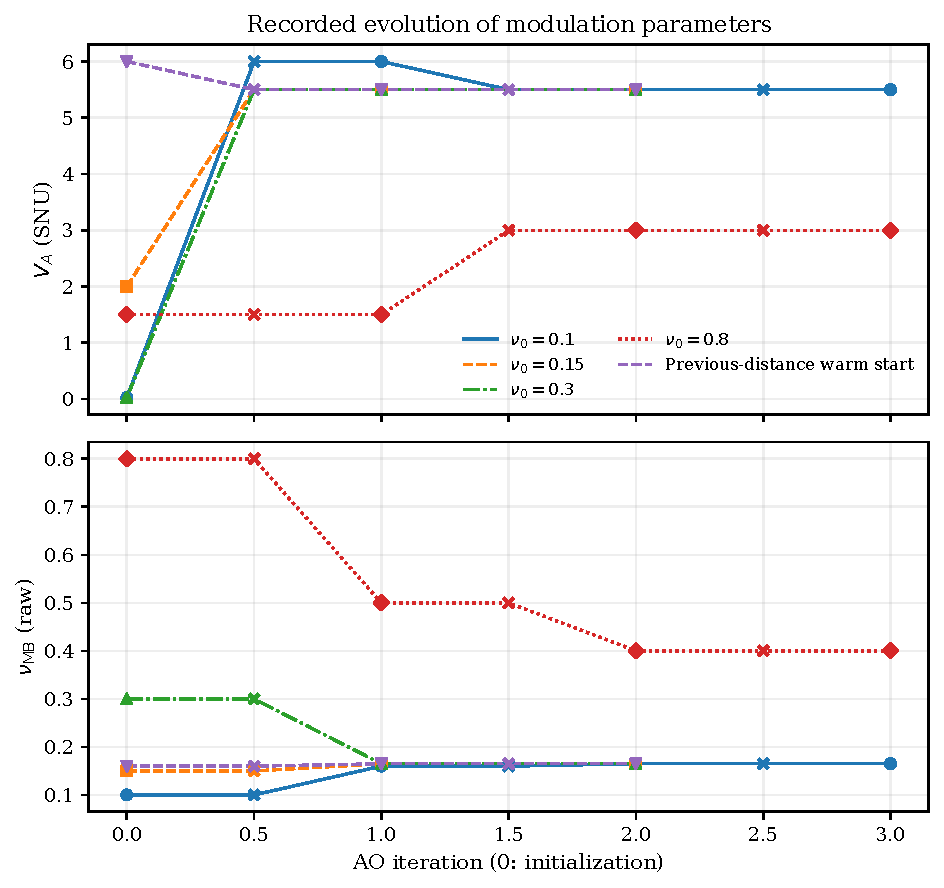
\includegraphics[width=\linewidth]{ao_parameter_evolution.pdf}
 \caption{Actual evolution of $V_A$ and $\nu_{\rm MB}$ for the same starts.
 The half-step records show that P1 updates variance with shaping fixed;
 P2 then updates shaping with the new variance fixed. Lines guide the eye
 between recorded events, not interpolated objective evaluations.}
 \label{fig:ao-parameters}
\end{figure}

\subsection{Distance comparison}
Figure~\ref{fig:skr-distance} compares the stored optimized-Uniform results,
the fixed MB reference and the AO-selected MB results on the established
distance grid. The full-angle divergence is $10~\mu$rad, receiver diameter
$0.55$ m, beam waist $0.0986760647169751$ m, HAP/UAV altitudes $20/1$ km,
wavelength $1550$ nm and zenith atmospheric transmittance $0.92$.
Optical adaptive optics and phase noise are off; channel excess noise is
$0.0186$ SNU and reconciliation efficiency is $0.95$. Optical adaptive optics
is distinct from the alternating-optimization algorithm.
The fixed MB curve uses its single stored binary64 reference pair,
$(\nu_{\rm MB},V_A)=(0.2,1.3833230302980657)$, at every distance.
The Uniform curve is the best available result of its historical exact
adaptive search, not a newly certified unconstrained continuous maximum.
On every evaluated distance, the AO-selected finite-catalog result exceeds
the fixed MB reference. At the reference distance, the fixed MB value is
$0.05268768994955189$ bits/use, giving a best-found SKR ratio of approximately
$1.4801$. At $40$ km the selected pair is
$(0.15,3.5548673904962893)$ and the SKR is $0.00225888275226813$ bits/use,
compared with $0.0016507968216343365$ bits/use for fixed MB (ratio approximately
$1.3684$). These comparisons concern the stored evaluated samples and the
declared unconstrained modulation experiment, not extrapolated range or an
energy-constrained hardware throughput claim.

\begin{figure}[t]
 \centering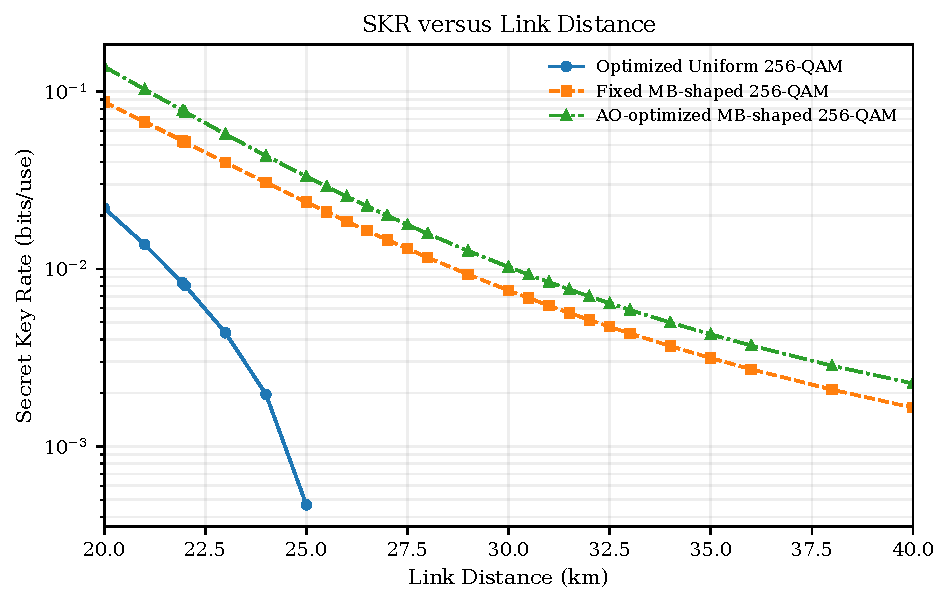
\includegraphics[width=\linewidth]{skr_vs_distance.pdf}
 \caption{SKR versus link distance from compatible stored exact-source
 numerical results. AO-optimized MB denotes the best validated finite-catalog
 result currently available, not a mathematically certified continuous global
 optimum. Only strictly positive samples are displayed on a base-10 logarithmic
 axis: Uniform ends at its last positive evaluated point, $25$ km, while both
 MB curves extend through $40$ km. No zero crossing is interpolated and no
 non-positive value is changed into a positive one.}
 \label{fig:skr-distance}
\end{figure}

\subsection{Remaining numerical evidence}
The reference P1 bracket is $[5.4875,5.5125]$, of width $0.025$.
Its active paired midpoints are $(0.165,5.49375)$ and $(0.165,5.50625)$.
The P2 bracket at $V_A=5.5$ is $[0.1625,0.16562500000000002]$;
its active requests are $(0.16375,5.5)$ and
$(0.16531250000000003,5.5)$. No coordinate search in the selected results is
fully completed. Obtaining a single midpoint would not establish convergence;
the original AO logic must determine the next incumbent and requests after
each validated evaluation. The four-stage cap, persistent unresolved flag,
remote-domain coverage, uniform-endpoint coverage and total objective-error
control remain relevant limitations. Consequently the appropriate claims are
finite-catalog maximization and reproducible best-found numerical performance,
without continuous/global optimality or expanded security claims.

Conditionally keeping the incumbent fixed, midpoint halving of the current P1
and P2 radii to $10^{-6}$ would require 14 and 12 levels, respectively, rather
than the four stages permitted in one inner call. These are geometric planning
counts, not observed iterations or guarantees. Further moments can improve the
best-found objective, but do not by themselves remove the implemented
refinement-cap and stagnation limitations; those settings are not changed here.
